\documentclass[10pt,a4paper, landscape, english]{article}
\usepackage[utf8]{inputenc}
\usepackage[left=2cm,right=2cm,top=2cm,bottom=2cm]{geometry}
\usepackage{babel}

% Will change name of weekdays
\usepackage{translator}

\usepackage[T1]{fontenc}


\author{Tim Benedikt Herbstrith}
\pagestyle{empty}

\usepackage{tikz}
\usepackage{pgfcore}
\usepackage{pgfcalendar}


% Setup of lengths
\newcommand{\widthofday}{4}
\newcommand{\lengthofhour}{1}
\newcommand{\entrytextwidth}{3.5}

% Set the first and last hour of the day
\newcommand{\firstH}{8}
\newcommand{\lastH}{18}

% TikZ style to display different subcalendars
\tikzstyle{sem}=[fill=black!80, text=white]


% Macros for drawing calendar entries, short version will only print the title of the entry
\newcommand{\calentry}[6][]{
	\filldraw[black!20, rounded corners, #1] ({day(#2,-1)},{time(#3)}) rectangle ({day(#2,1)},{time(#4)});%
	\node[anchor=north, font=\scriptsize, text width=\entrytextwidth cm, #1] at ({day(#2,0)},{time(#3)}) {#3\\ \textbf{#5}\\ #6};%
}
\newcommand{\shortcalentry}[5][]{
	\filldraw[black!20, rounded corners, #1] ({day(#2,-1)},{time(#3)}) rectangle ({day(#2,1)},{time(#4)});%
	\node[font=\scriptsize, text width=\entrytextwidth cm, #1] at ({day(#2,0)},{halftime(#3,#4)}) {\textbf{#5}};%
}

\begin{document}
\begin{center}

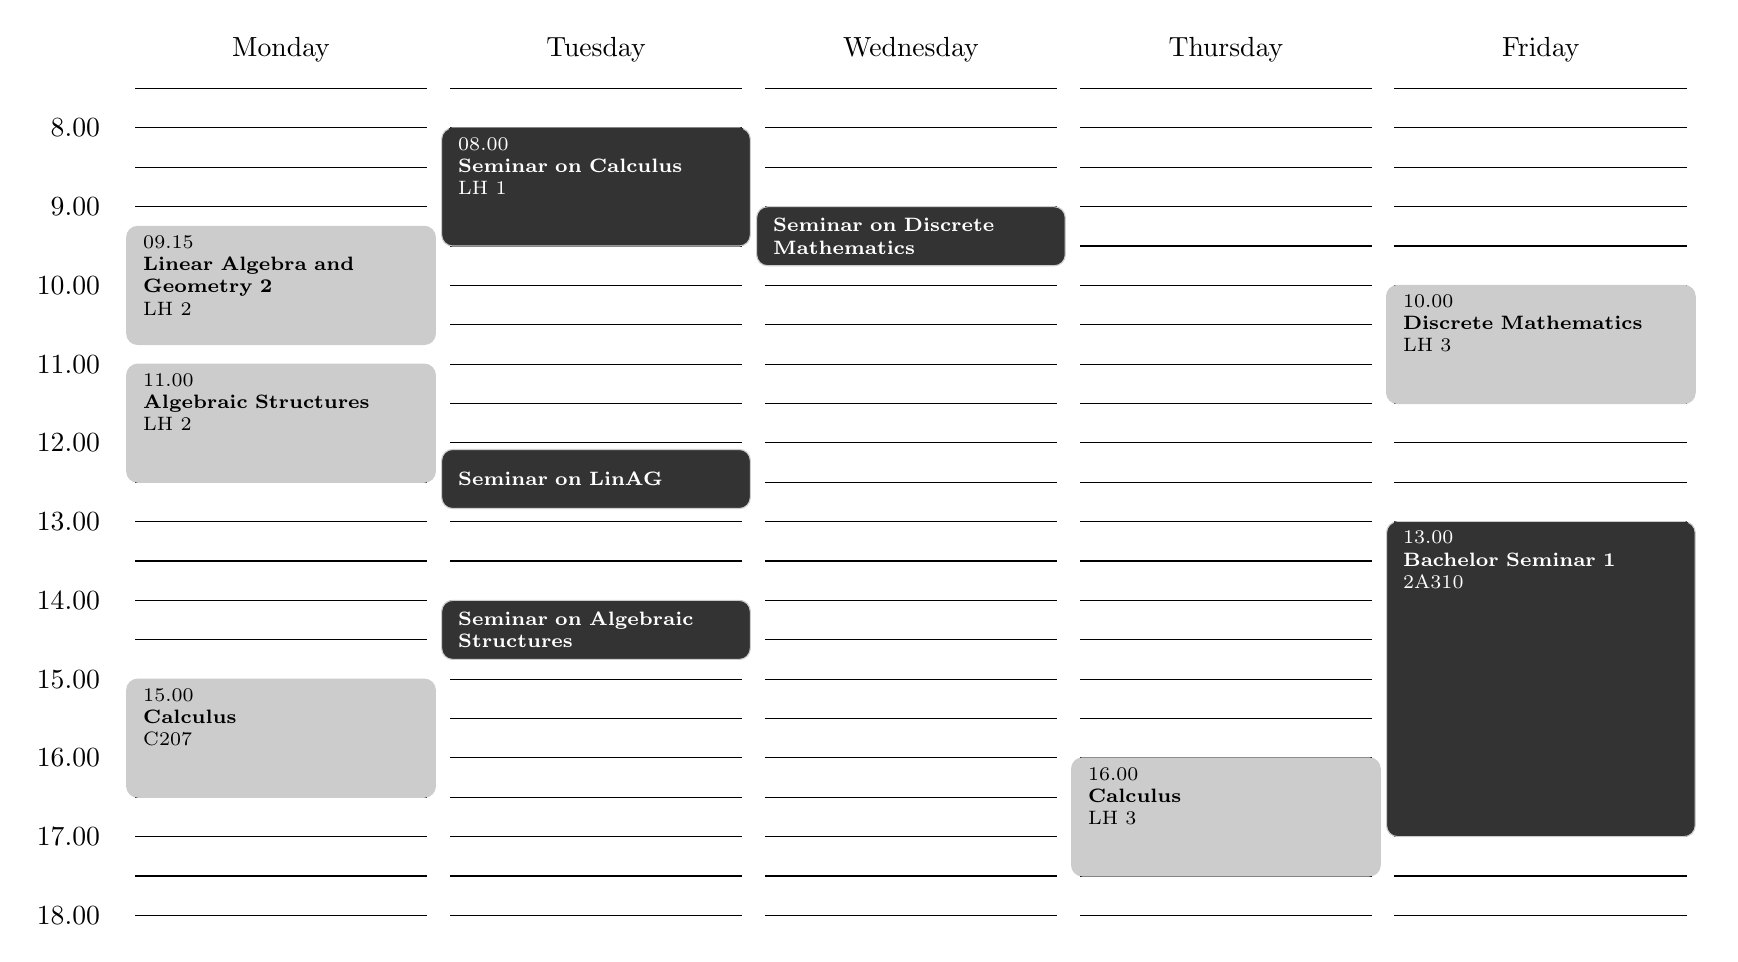
\begin{tikzpicture}[x=\widthofday cm, y=\lengthofhour cm]

% Offset for the rectangle marking appointments
\pgfmathsetmacro{\offsetForAppointment}{+0.01}

% Converts the integer marking the day of the week to a coordinate.
% The second argument specifies wheter the left (-1), the base (0) or the right end of the column is returned.
\pgfmathdeclarefunction{day}{2}{%
	\pgfmathparse{-#2*\offsetForAppointment+#1-(1-#2)/2}%
}

% Converts a given time (hh.mm) to a length. \firstH is converted to 0.
\pgfmathdeclarefunction{time}{1}{%
	\pgfmathparse{\firstH-(floor(#1)+(#1-floor(#1))/0.6)}%
}

% Finds the mean of the duration of the appointment. Used in \shortcalentry.
\pgfmathdeclarefunction{halftime}{2}{%
	\pgfmathparse{(time(#1)+time(#2))/2}%
}
	
% Draws the timtables grid
\foreach \hour in {\firstH,...,\lastH}
	\draw (0,\firstH-\hour) node[left=5] {\hour.00} -- (5,\firstH-\hour)  (0,\firstH+0.5-\hour) -- (5,\firstH+0.5-\hour);
\foreach \day in {0,...,5}
	\draw[line width=8pt,white] (\day,0.6) -- (\day,\firstH-\lastH -0.1);
	
% Prints days of the week, first day of the week (1) is Monday!
\foreach \day in {0,...,4}
	\node at (0.5+\day,1) {\pgfcalendarweekdayname{\day}};

% Here are the actual entries of our timetable
\calentry{1}{09.15}{10.45}{Linear Algebra and Geometry 2}{LH 2}
\calentry{1}{11.00}{12.30}{Algebraic Structures}{LH 2}
\calentry{1}{15.00}{16.30}{Calculus}{C207}

\calentry[sem]{2}{08.00}{9.30}{Seminar on Calculus}{LH 1}
\shortcalentry[sem]{2}{12.05}{12.50}{Seminar on LinAG}{LH 1}
\shortcalentry[sem]{2}{14.00}{14.45}{Seminar on Algebraic Structures}{C209}

\shortcalentry[sem]{3}{09.00}{09.45}{Seminar on Discrete Mathematics}{C209}

\calentry{4}{16.00}{17.30}{Calculus}{LH 3}

\calentry{5}{10.00}{11.30}{Discrete Mathematics}{LH 3}
\calentry[sem]{5}{13.00}{17.00}{Bachelor Seminar 1}{2A310}


\end{tikzpicture}

\end{center}
\end{document}